\begin{subsectionframemod}{Cross-Domain Few-Shot Object Detection}

    \metroset{block=fill}
    \begin{alertblock}{Détection d'objets few-shot cross-domain}
        En détection d'objets few-shot cross-domain, on utilise deux datasets de domaines différents :
        un dataset source avec beaucoup de données annotées et un dataset cible, plus restreint.
        L'objectif est d'exploiter le dataset source pour améliorer la détection sur le dataset cible.
        Le modèle doit s'adapter à la fois à de nouvelles classes et à des images inédites, rendant la tâche plus complexe.
    \end{alertblock}

    \only<1>{
        \begin{figure}
            \centering
            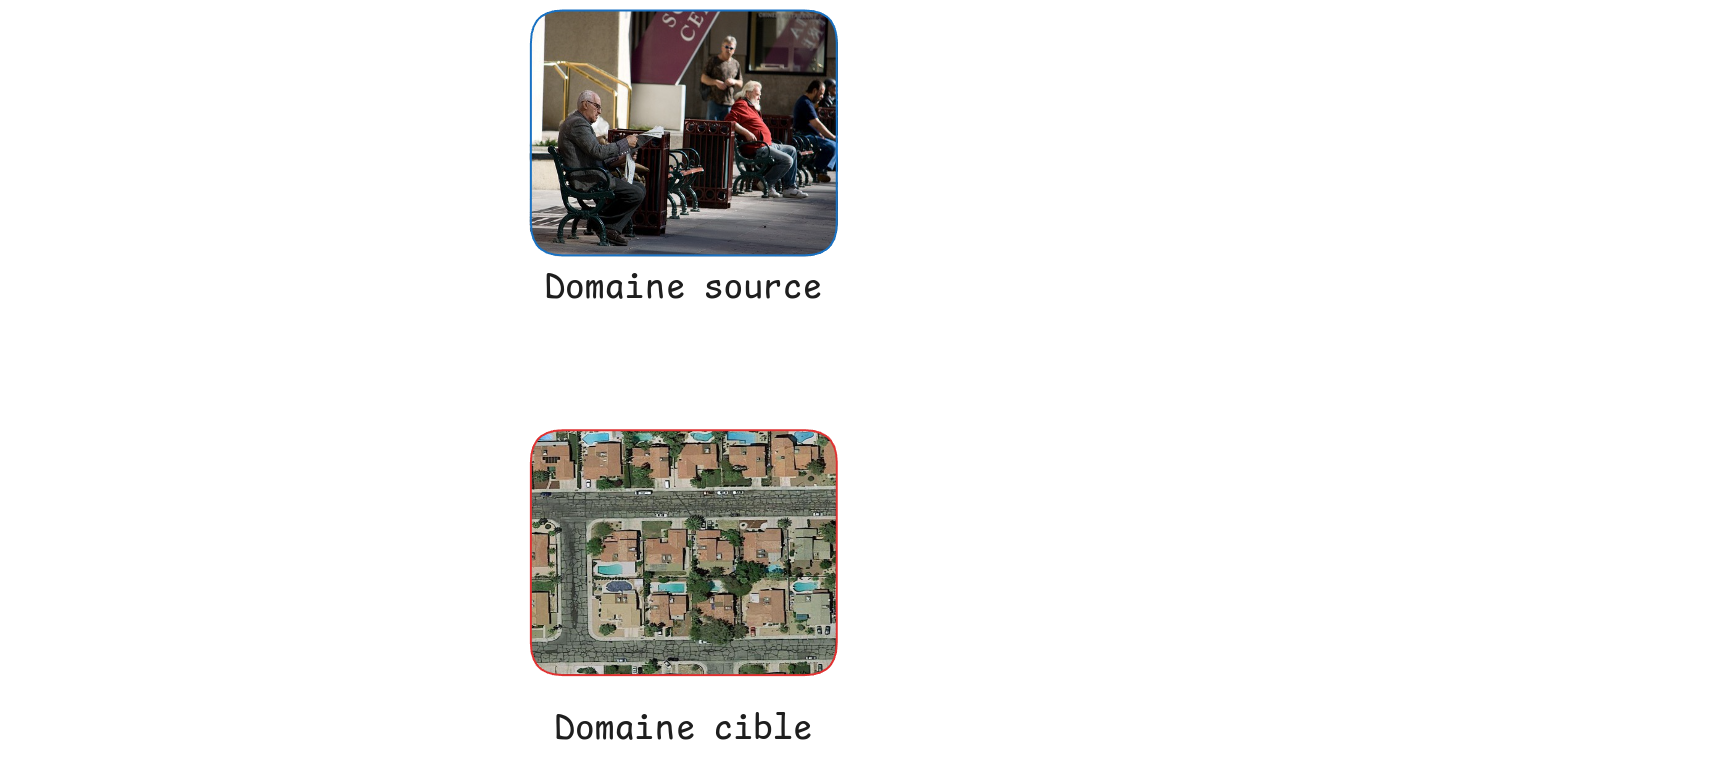
\includegraphics[width=\textwidth]{Figures/cross_domain}
        \end{figure}
    }
    \pause
    \only<2>{
        \begin{figure}
            \centering
            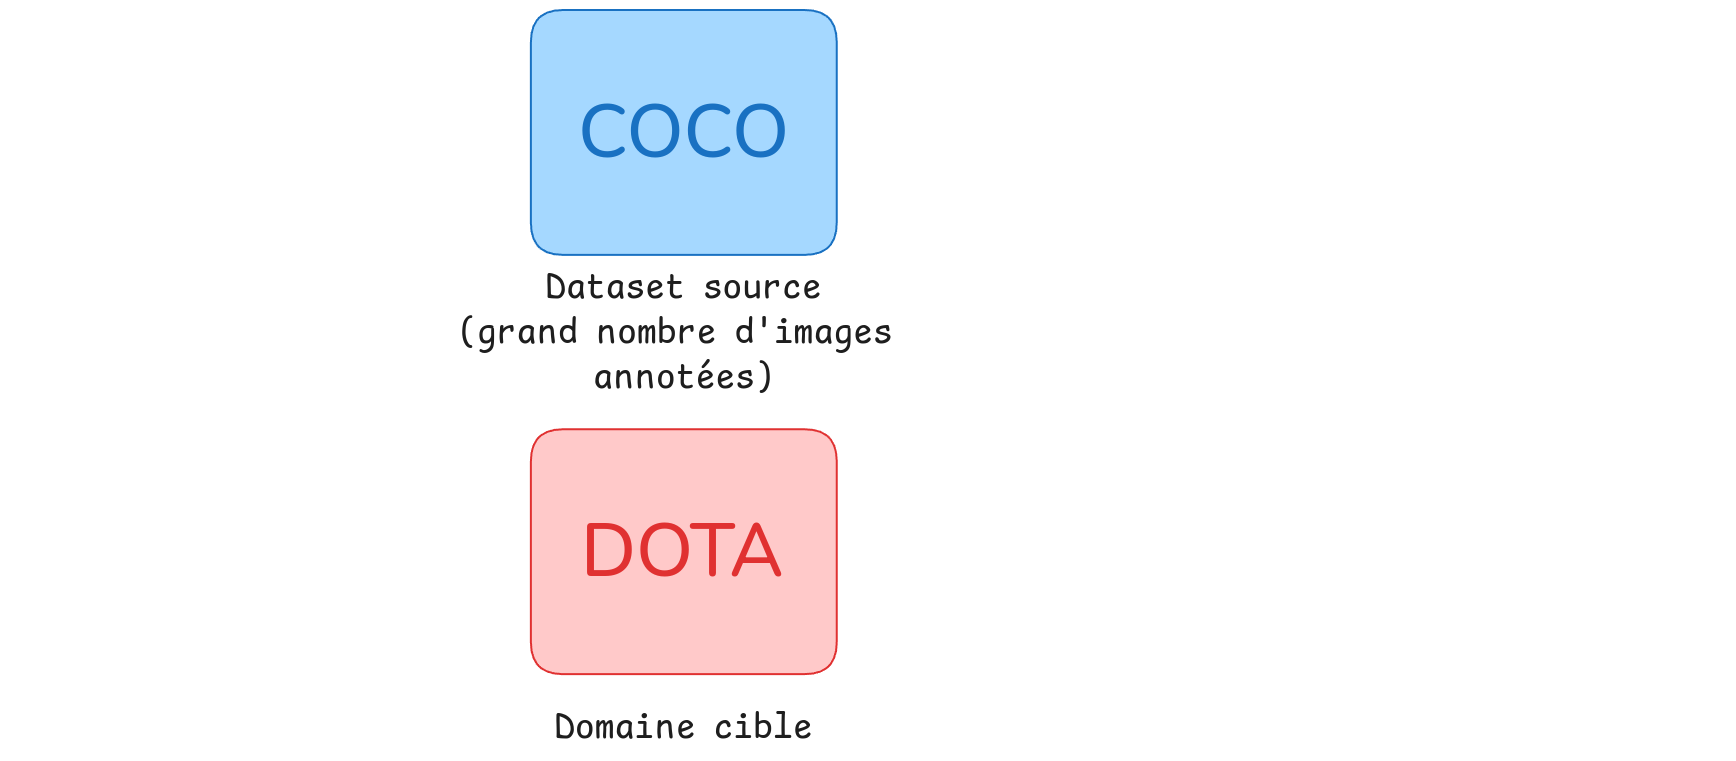
\includegraphics[width=\textwidth]{Figures/cross_domain_0}
        \end{figure}
    }
    \pause
    \only<3>{
        \begin{figure}
            \centering
            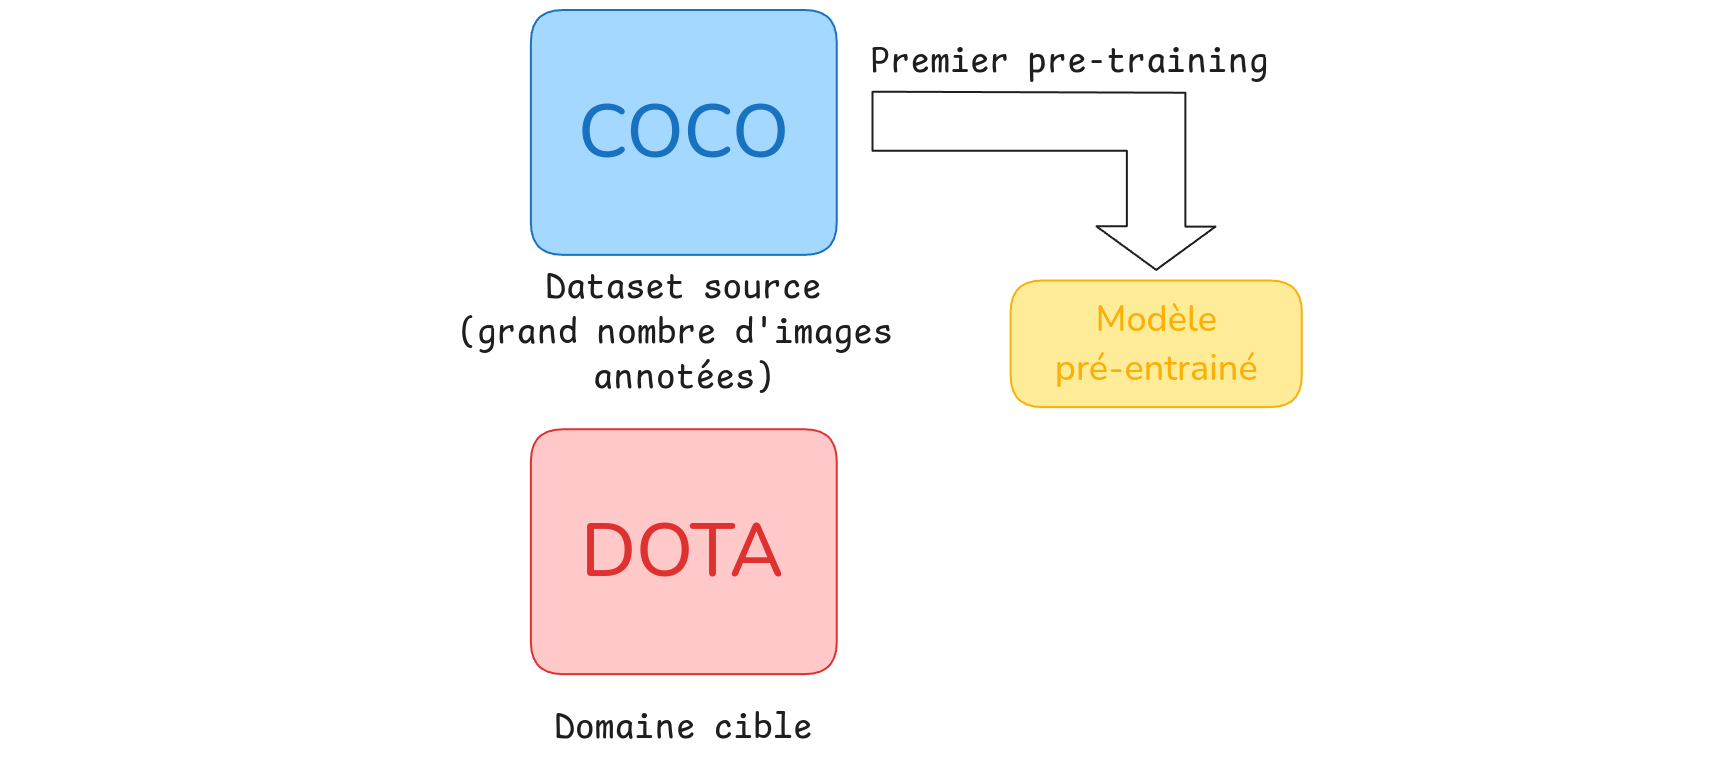
\includegraphics[width=\textwidth]{Figures/cross_domain_1}
        \end{figure}
    }
    \pause
    \only<4>{
        \begin{figure}
            \centering
            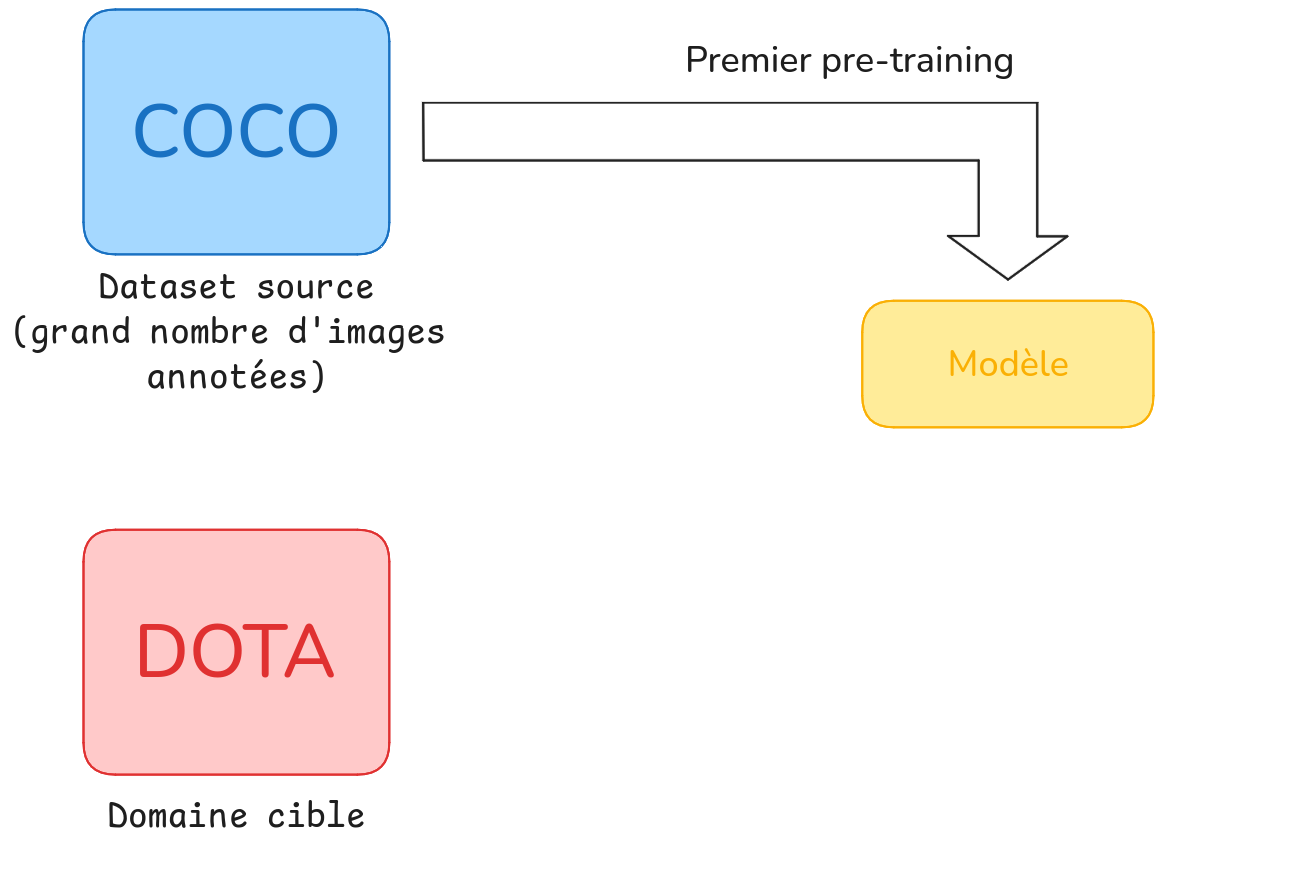
\includegraphics[width=\textwidth]{Figures/cross_domain_2}
        \end{figure}
    }
    \pause
    \only<5>{
        \begin{figure}
            \centering
            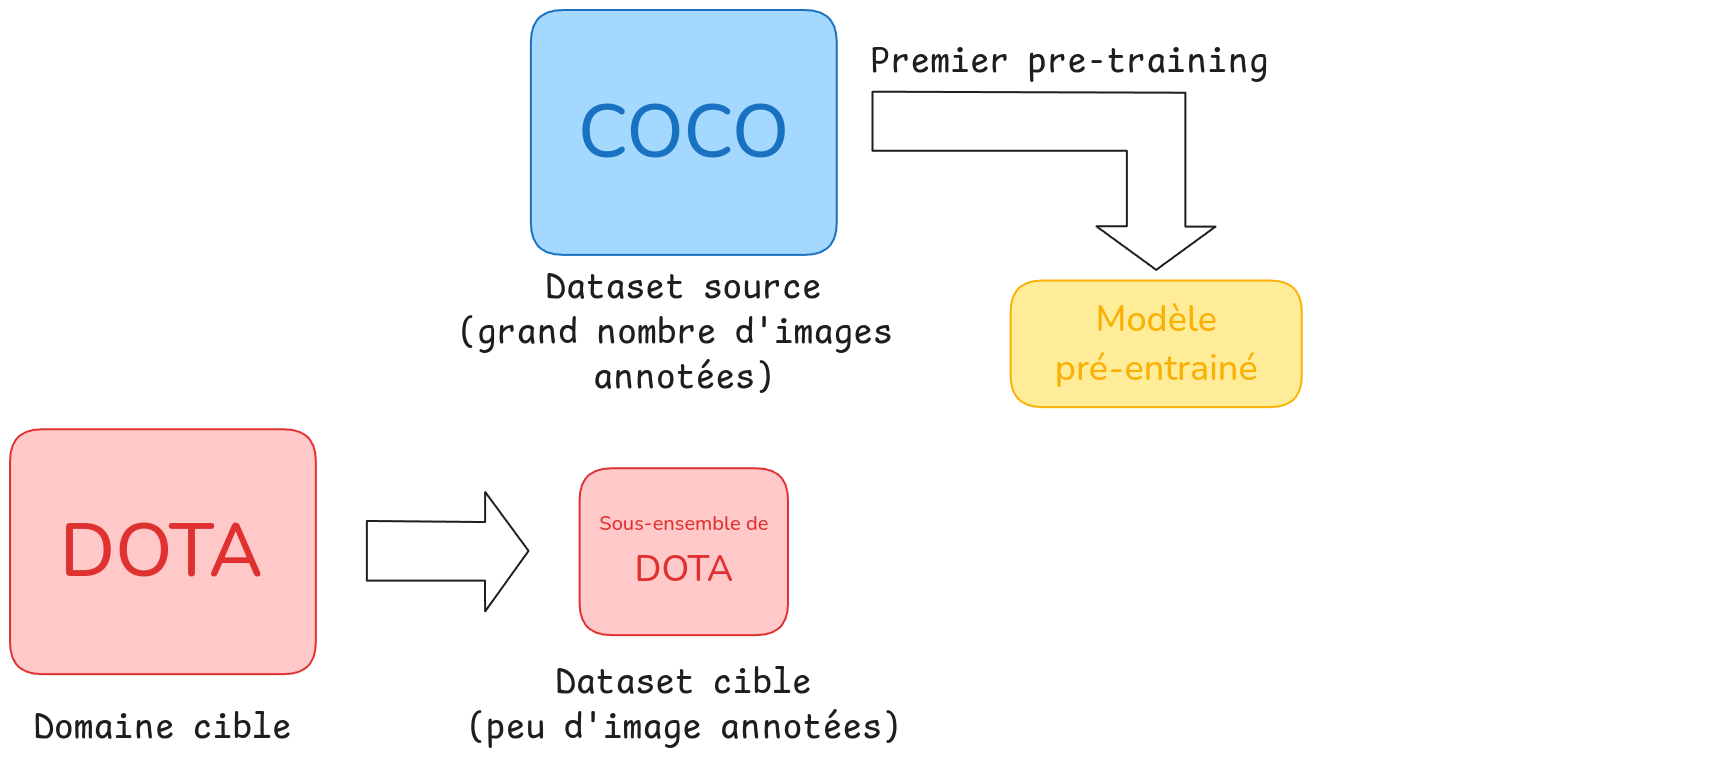
\includegraphics[width=\textwidth]{Figures/cross_domain_3}
        \end{figure}
    }
    \pause
    \only<6>{
        \begin{figure}
            \centering
            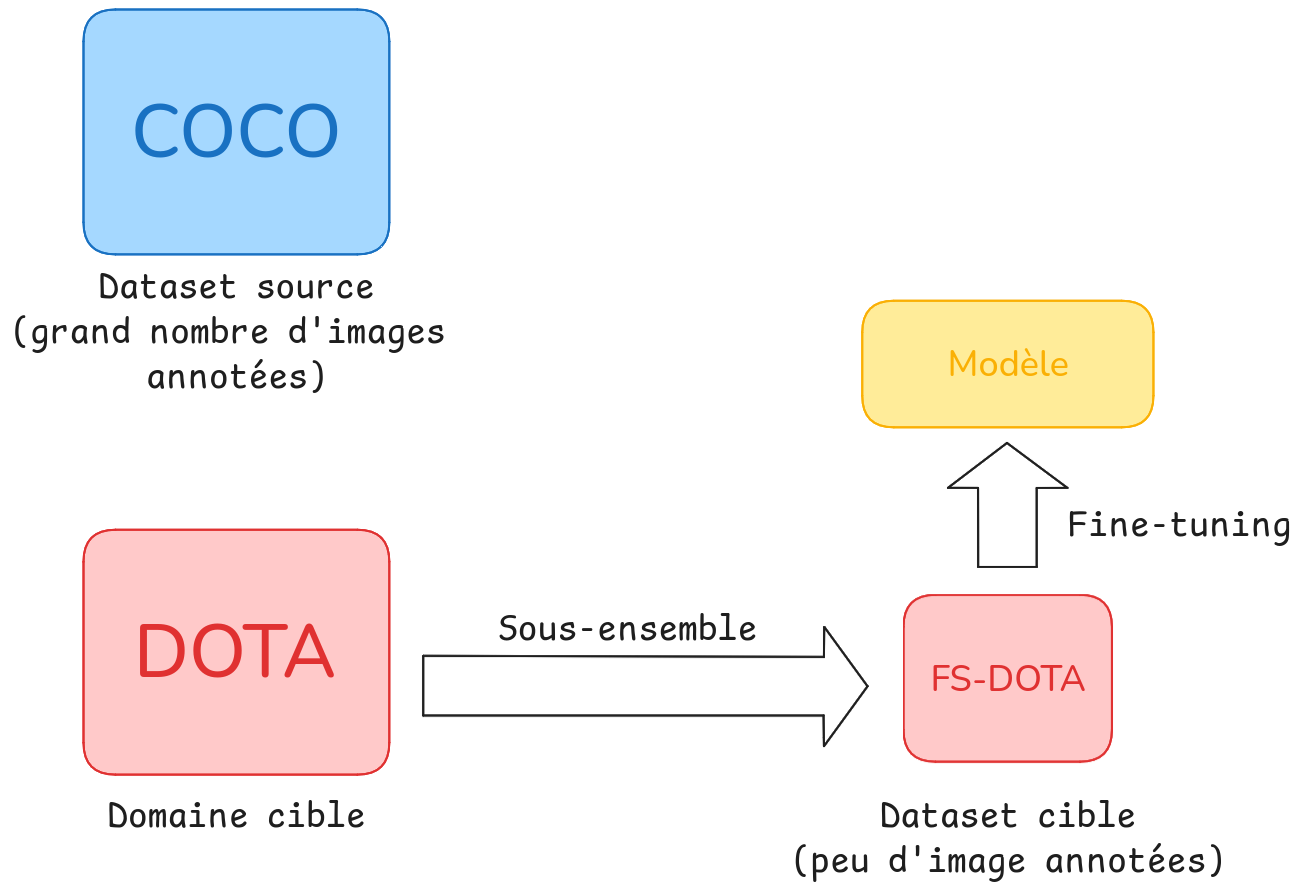
\includegraphics[width=\textwidth]{Figures/cross_domain_4}
        \end{figure}
    }

\end{subsectionframemod}